\section{Methodology}

We evaluated seven AI models (Claude (Anthropic), AWS Claude, Google Gemini, Gemma2, Gemma7, Llama3, and Mixtral) across three distinct marine regions: the Northern Territory (tropical waters), South East Inshore (temperate coastal waters), and South East Offshore (temperate oceanic waters). We defined each region using shapefiles containing precise geographical boundaries, which we converted to GeoJSON format for processing (Figure \ref{fig:validation_regions}).

\begin{figure}[H]
    \centering
    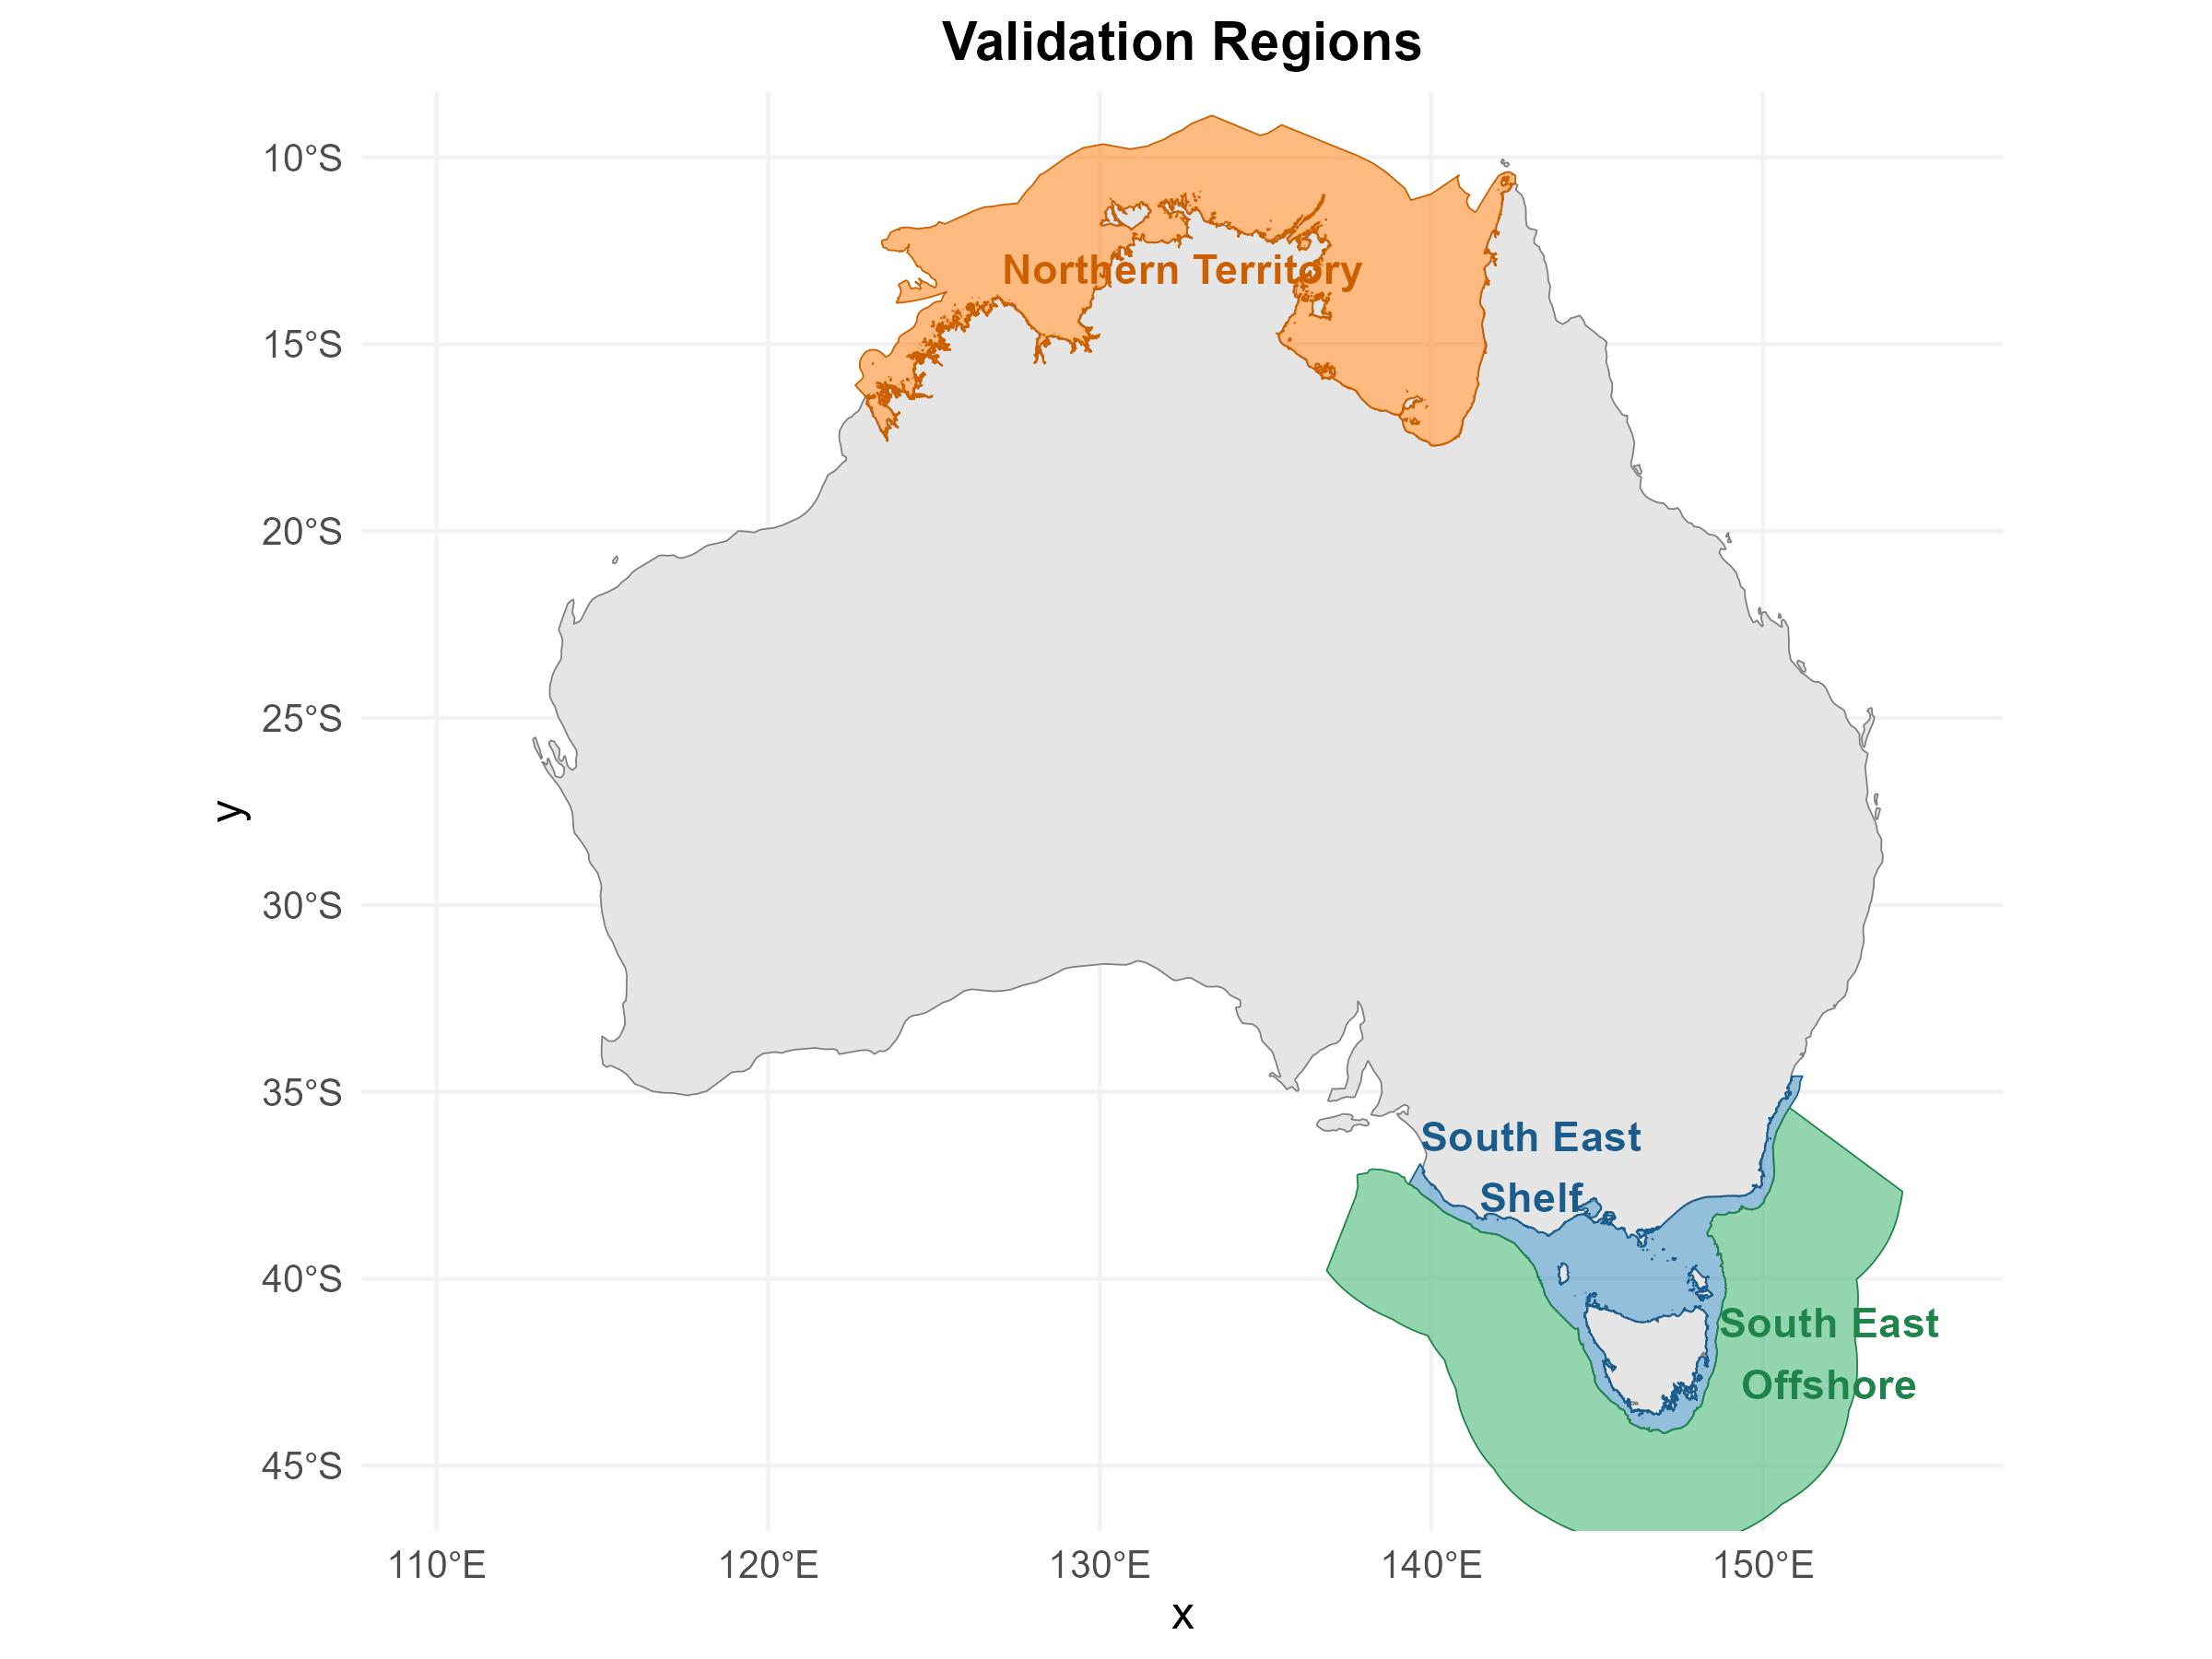
\includegraphics[width=\textwidth]{validation_regions.png}
    \caption{Validation regions used in the study: Northern Territory (tropical), South East Inshore (temperate coastal), and South East Offshore (temperate oceanic).}
    \label{fig:validation_regions}
\end{figure}

\subsection{Regional Ecosystem Understanding}
To assess AI models' comprehension of regional marine ecosystems, we employed a standardized prompting protocol (see Supplementary Material, AI Prompting Protocol). For each region, we first extracted geographic extents from the GeoJSON files to define the study area boundaries. We then prompted each model to provide detailed ecosystem descriptions encompassing geographic location, notable features, marine environment type, oceanographic conditions, habitat types, and key ecological characteristics.

We evaluated these AI-generated descriptions through multiple criteria:
\begin{itemize}
    \item Comprehensiveness of physical and biological characteristics
    \item Accuracy compared to known oceanographic patterns
    \item Alignment with regional ecological surveys
    \item Consistency with documented biodiversity patterns
    \item Accuracy of described seasonal dynamics
\end{itemize}

\subsection{Functional Group Generation Consistency}
We implemented an iterative validation protocol to assess the consistency of functional group generation. The process involved a two-stage approach for each region and AI model combination. First, we provided the AI model with the validated ecosystem description and a comprehensive template of possible functional groups (see Supplementary Material, Grouping Template). This template served as a reference point but did not constrain the models, which could create new groups or modify existing ones based on regional characteristics.

The group generation process followed specific ecological criteria:
\begin{itemize}
    \item Groups could represent individual species or collections of species sharing similar ecological functions
    \item Species were grouped based on similar growth rates, consumption rates, diets, habitats, and predators
    \item Groupings prioritized ecological niche similarity over taxonomic relationships
    \item Higher resolution groupings were maintained for species related to the research focus
    \item Broader functional groups were used for species with less direct relevance to the study objectives
\end{itemize}

For each region-model combination, we conducted five independent iterations. Each iteration generated a complete set of functional groups, with results stored in a standardized JSON format including detailed descriptions of each group's ecological role. We tracked group occurrence across iterations and created group occurrence matrices. To quantify consistency, we calculated a consistency score for each functional group using:

\[
\text{Consistency Score} = \frac{\text{Number of occurrences of group}}{\text{Total number of iterations}}
\]

We generated heatmaps to visualize consistency patterns across models and regions.

\subsection{Ecological Validity Assessment}
We evaluated the ecological validity of AI-generated functional groups by analyzing their adherence to established ecological principles. For each generated group set, we assessed:
\begin{itemize}
    \item Coverage across all major trophic levels
    \item Representation of key ecological roles
    \item Appropriateness of species groupings based on ecological function
    \item Adaptation to region-specific characteristics
    \item Alignment with known trophic interactions
\end{itemize}

\subsection{Technical Implementation}
The validation framework employed several Python scripts:
\begin{itemize}
    \item validate\_ai\_groupings.py: Core validation script
    \item group\_species\_utils.py: Group generation and processing
    \item ask\_AI.py: AI model interactions
\end{itemize}

We used pandas for data manipulation, seaborn and matplotlib for statistical visualization, and geopandas for geographical data processing. All validation runs were stored in timestamped directories, preserving raw results as JSON files, ecosystem descriptions, group matrices as CSV files, and calculated consistency metrics.
